Différents tests de validation ont été effectués tout au long du projet afin de s'assurer du bon fonctionnement de l'application. Ces tests pourront être refaits par la suite en décommentant les $\sharp$define nécessaires, et pourront donc être réutilisés par des étudiants reprenant ce projet.

\subsection{Latence}

\begin{figure}[!h]
\centering
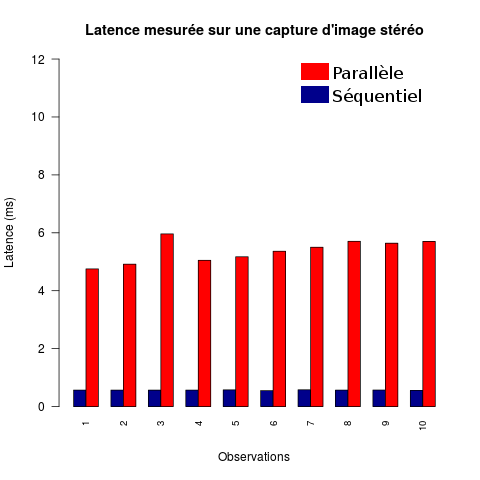
\includegraphics[width=\textwidth, height=10cm]{Modules/Picture/latence.png}
\caption{Latence}
\label{latence}
\end{figure}

\begin{figure}[!h]
\centering
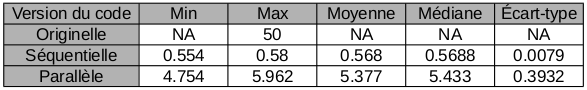
\includegraphics[width=\textwidth, height=2cm]{Modules/Picture/tableauLatence.png}
\caption{Comparaison de la latence}
\end{figure}

\newpage

La latence est une caractéristique incontournable de notre projet, le client nous ayant précisé plusieurs fois que c'était très important qu'il y ait le moins de décalage possible entre les deux vidéos. Plus le décalage est grand et moins la reconstruction en 3D par la suite sera précise. Nous avons donc mesuré précisément le temps qui sépare deux frames dans le code. 

Ce diagramme en bâton (Figure \ref{latence}) montre cette latence. Elle est plus importante avec le parallélisme qu'avec le programme séquentiel. Il faudra donc que le client pèse le pour et le contre sur la méthode qu'il préfère utiliser. Avec le parallelisme, le nombre de caméra pourra être augmenté (de façon raisonnable) sans chute de fps, car chaque coeur de la machine s'occupera d'une caméra particulière, par contre, la latence est plus importante : 5 à 6 ms. Avec la version séquentielle du code, la latence est plus que minime : 1/2 millième de seconde environ. Par contre, séquentiellement, comme on lance les acquisitions les unes après les autres, plus il y a de caméras, plus celles qui sont lancées en dernier auront de décalage avec la première.

\subsection{FPS}

\begin{figure}[!h]
\centering
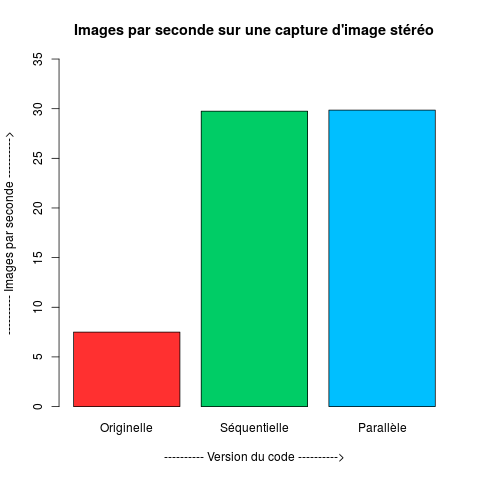
\includegraphics[width=\textwidth, height=10cm]{Modules/Picture/fps.png}
\caption{FPS}
\label{fps}
\end{figure}

\begin{figure}[!h]
\centering
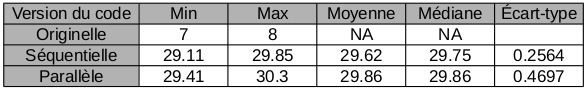
\includegraphics[width=\textwidth, height=2cm]{Modules/Picture/tableauFPS.png}
\caption{Comparaison des FPS}
\end{figure}

L'augmentation du nombre de FPS était un des objectifs principaux de notre TER. En effet, le groupe précédent n'arrivaient qu'à enregistrer des images à la vitesse de 7/8 FPS, ce qui ne permettait pas une reconstruction optimale. Comme on peut le voir sur la Figure \ref{fps}, nous faisons de l'acquisition à 30 FPS constants, en parallèle comme en séquentiel. Cependant, nous pensons qu'il faut privilégier le code fait en parallèle, car il est plus robuste à l'ajout de caméras futures.

